For the video model, we selected a transformer-based architecture: ViVit \cite{DBLP:journals/corr/abs-2103-15691}. This choice was motivated by the notable performance of transformers in single-image classification, the ability of these architectures to capture long-term dependencies through attention mechanisms, and the demonstrated effectiveness of ViVit as a modern, accessible model achieving promising results \cite{DBLP:journals/corr/abs-2103-15691}.

The specific ViVit model being used was Google’s Vivit-b-16x2-kinetics400, which features a base backbone comprising 12 transformer layers, each with a 12-head self-attention block \cite{DBLP:journals/corr/abs-2103-15691}. ViVit captures spatio-temporal information by structuring data into `tubes' across three dimensions: height, width, and temporal, which in this case were set to 16, 16, and 2, respectively \cite{DBLP:journals/corr/abs-2103-15691}. This model was pretrained on the Kinetics-400 dataset and only the weights of the final layer were modified during training.

% Commented as requested by the teacher
% \begin{figure}[H]
%     \centering
%     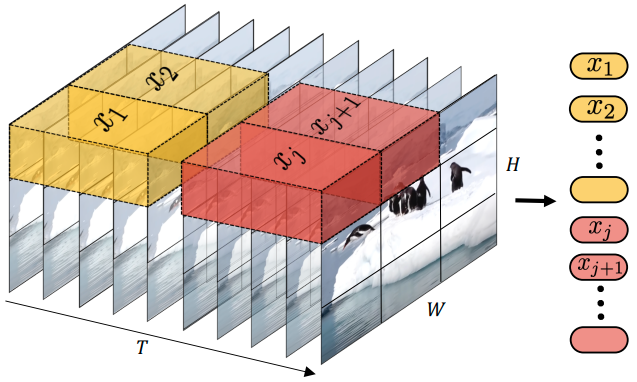
\includegraphics[width=0.8\linewidth]{imgs//models/vivit_tubes.png}
%     \caption{ViVit `tubes' representation \cite{DBLP:journals/corr/abs-2103-15691}.}
%     \label{fig:vivit_tubes}
% \end{figure}

% Commented to make it more concise
% ViVit required additional data handling to transform the images into a readable structure. This involved converting each patient's sequence of slices into a tensor, which was then added to a new dataset along with its corresponding label (positive or negative). The dataset was subsequently saved as a file, allowing for reuse and eliminating the need to repeat this computationally intensive step.

The model was used with the following parameters, which yielded optimal performance: a validation proportion of 0.3, a learning rate of 0.000005, and a maximum of 20 epochs with early stopping to prevent overfitting.